\documentclass[handout]{beamer}
% \documentclass{beamer}

%%
%%
%%
% From http://tex.stackexchange.com/questions/2072/beamer-navigation-circles-without-subsections
% Solution #2 or 3:
% \usepackage{etoolbox}
% \makeatletter
% % replace the subsection number test with a test that always returns true
% \patchcmd{\slideentry}{\ifnum#2>0}{\ifnum2>0}{}{\@error{unable to patch}}%
% \makeatother
% Solution #1:
\usepackage{remreset}% tiny package containing just the \@removefromreset command
\makeatletter
%\@removefromreset{subsection}{section}
%\makeatother
%\setcounter{subsection}{1}




\usepackage{etex}
\usepackage{pgf}
\usepackage{tikz}
\usepackage{url}
\usepackage{amsmath}
\usepackage{color}
% \definecolor{red}{rgb}{1,0,0}
\usepackage{ulem}
% \usepackage{booktabs}
\usepackage{colortbl,booktabs}
\renewcommand*{\thefootnote}{\fnsymbol{footnote}}
\usepackage{fancybox}
\usepackage[framemethod=TikZ]{mdframed}
\mdfdefinestyle{FactStyle}{%
  outerlinewidth=0.5,
  roundcorner=1pt,
  leftmargin=1cm,
  linecolor=blue,
  outerlinecolor=blue!70!black,
  backgroundcolor=yellow!40
}
\usepackage{cancel}

  \newcommand\Warning{%
    \makebox[2.4em][c]{%
      \makebox[0pt][c]{\raisebox{.2em}{\Large!}}%
      \makebox[0pt][c]{\color{red}\Huge$\bigtriangleup$}}}%

\usepackage{stackengine}
\usepackage{scalerel}
\usepackage{xcolor}
  \newcommand\dangersign[1][2ex]{%
    \renewcommand\stacktype{L}%
    \scaleto{\stackon[1.3pt]{\color{red}$\triangle$}{\tiny !}}{#1}%
  }



\usepackage{dcolumn}
\newcolumntype{d}[1]{D{.}{.}{#1}}

% From
% http://tex.stackexchange.com/questions/109900/how-can-i-box-multiple-aligned-equations
\usepackage{empheq}
\usepackage{tcolorbox}  \newtcbox{\othermathbox}[1][]{%
  nobeforeafter, tcbox raise base, 
  colback=black!10, colframe=red!30, 
  left=1em, top=0.5em, right=1em, bottom=0.5em}

\newcommand\blue{\color{blue}}
\newcommand\red{\color{red}}
\newcommand\green{\color{green!75!black}}
\newcommand\purple{\color{purple}}
\newcommand\bluegreen{\color{blue!75!green}}
\newcommand\orange{\color{orange}}
\newcommand\redgreen{\color{red!50!green}}
\newcommand\grey{\color{black}}
\newcommand\gap{\vspace{.1in}}
\newcommand\nb{${\red\bullet}\ $}
\newcommand\halfgap{\vspace{.05in}}
\newcommand\divideline{\line(1,0){352}}
\usepackage{marvosym} % for \Smiley

\newcommand{\bluealert}[1]{{\blue\textbf{#1}}}

% \usepackage{beamerthemesplit} %Key package for beamer
\usetheme{Singapore}
% \usetheme{Szeged}
% \usetheme{Garfield}
% \usetheme{CambridgeUS}
% \usenavigationsymbolstemplate{} %Gets rid of slide navigation symbols


\setbeamercolor{separation line}{use=structure,bg=structure.fg!50!bg}
% \begin{beamercolorbox}[colsep=0.5pt]
%   {upper separation line foot}
% \end{beamercolorbox}



\makeatletter
\setbeamertemplate{footline}
{
  \leavevmode%
  \hbox{%
% \begin{beamercolorbox}[colsep=0.5pt]
%   {upper separation line foot}
% \end{beamercolorbox}


  \begin{beamercolorbox}[wd=.5\paperwidth,ht=2.25ex,dp=2ex,colsep=0.5pt]%
    {upper separation line foot}
    \usebeamerfont{author in head/foot}%
    \hspace*{2ex}\insertshortdate:\ \insertshorttitle
  \end{beamercolorbox}%
  \begin{beamercolorbox}[wd=.5\paperwidth,ht=2.25ex,dp=2ex,right]{title in head/foot}%
    \usebeamerfont{title in head/foot}
    {\insertshortauthor}\hspace*{2ex}
  \end{beamercolorbox}}%
  % \begin{beamercolorbox}[wd=.333333\paperwidth,ht=2.25ex,dp=2ex,right]{date in head/foot}%
  %   \usebeamerfont{date in head/foot}\insertshortdate{}\hspace*{2em}
  %   \insertframenumber{} / \inserttotalframenumber\hspace*{2ex} 
  % \end{beamercolorbox}%
  \vskip0pt%
}
\makeatother

\usetikzlibrary{decorations.markings}
\usetikzlibrary{arrows}


\title{Final Exam Review}
\author{Schley, UCSB Mathematics}
\date{March 15, 2017}
%\institute{}


\useinnertheme{default}

\usefonttheme{serif}
% \usecolortheme{rose}
% \usecolortheme{whale}
% \usecolortheme{orchid}
\usecolortheme{crane}
% \usecolortheme{dolphin}


%TEMPLATE
\setbeamertemplate{navigation symbols}{}

\setbeamertemplate{note page}[compress]

\setbeamertemplate{frametitle}{
  \vspace{0.5em}
  % \begin{centering}
  {\huge\blue\textbf{\textmd{\insertframetitle}}}
  \par
  % \end{centering}
}

% From http://tex.stackexchange.com/questions/7032/good-way-to-make-textcircled-numbers:
\newcommand*\circled[1]{\tikz[baseline=(char.base)]{\node[shape=circle,draw,fill=orange,inner sep=1pt] (char) {#1};}} 
% \renewcommand{\labelenumi}{\circled{\textbf{\arabic{enumi}}}}

\let\olddescription\description
\let\oldenddescription\enddescription
\usepackage{enumitem}
\let\description\olddescription
\let\enddescription\oldenddescription

% \usepackage[loadonly]{enumitem}
\setlist[enumerate,1]{label=\colorbox{orange}{\arabic*.},font=\bfseries}
%\setlist[enumerate,2]{label=\colorbox{blue!25}{(\alph*)},font=\bfseries}
% \setlist[enumerate,1]{label=\arabic*.,font=\bfseries}
\setlist[itemize,1]{label=\red$\bullet$}
\setlist[itemize,2]{label=\blue$\bullet$}

\newcommand\answer[1]{\fbox{#1}}
% \renewcommand\answer[1]{}

\newcommand{\antilog}{\operatorname{antilog}}

\newcommand{\instructor}{Nathan Schley ({\it Sh}+{\it lye})}
\newcommand{\officehours}{T R 11-11:50, T 3:45-4:35 Details on Gauchospace.}
\newcommand{\email}{schley@math.ucsb.edu}
\newcommand{\officeloc}{South Hall 6701}
\newcommand{\copyrightinfo}{2022\ Daryl Cooper, Peter M.\ Garfield, Ebrahim Ebrahim \& Nathan Schley}
    













\title{}
\title{Maxima \& Minima}
\date{June 2, 2017}


\begin{document}
\small

\section*{Administration}

\frame{
  \frametitle{Office Hours!}
  % \ \vspace*{0.25in}

  {\Large{}Instructor:}\\
  \ \hspace*{0.2in} Trevor Klar, \url{trevorklar@math.ucsb.edu}\\[0.25em]

  {\Large{}Office Hours:}\\
  \ \hspace*{0.2in} Mondays 2--3\textsc{pm}\\
  \ \hspace*{0.2in} Tuesdays 10:30--11:30\textsc{am}\\
  \ \hspace*{0.2in} Thursdays 1--2\textsc{pm}\\
  \ \hspace*{0.2in} or by appointment \\[0.25em]

  {\Large{}Office:}\\
  \ \hspace*{0.2in} South Hall 6431X (Grad Tower, 6th floor, blue side, first door on the right)\\[0.5em]

  \copyright\ 2017\ Daryl Cooper, Trevor Klar

  % \vspace*{2in}
}

\if0
\section{Concavity Review}
\frame{
  \frametitle{Review:}

  {\red(1)}\ Where is  $f(x)=3x^2+18x-4$ increasing?
  \begin{center}
    A\ $x < -3$
    \quad 
    B\ $x > -3$
    \quad 
    C\ $x < 3$
    \quad 
    D\ $x > 3$
    \quad 
    E\ $x=3$
    \quad
    \pause
    \fbox{B}
  \end{center}
  \bigskip

  {\red(2)}\ Where is $f(x)$ increasing?
  \begin{center}
    \includegraphics[scale=0.7]{Figures/concave4.pdf}
  \end{center}
  \begin{center}
    A\ $x<0$
    \quad 
    B\ $x>2$
    \quad
    C\ $x<2$
    \quad 
    D\ $0<x<2$
    \quad
    E\ $x>0$
    \quad
    \pause
    \fbox{D}
  \end{center}
  
}

\frame{
  \frametitle{Continuing Review}

  \begin{center}
    \only<1-4>{\includegraphics[scale=0.7]{Figures/concave4.pdf}}
    \only<5->{\includegraphics[scale=0.7]{Figures/concave5.pdf}}
  \end{center}

  {\red(3)} Where is $f''(x)<0$?
  \begin{center}
    A\ $1<x<3$
    \quad 
    B\  $x>3$
    \quad 
    C\ $x>2$
    \quad 
    D\ $0<x<2$
    \quad 
    E\ $x<1$
    \quad
    \uncover<2->{\fbox{A}}
  \end{center}
  \bigskip

  \uncover<3->{%
  {\red(4)}\ Where is $f'(x)$ decreasing?
  \begin{center}
    A\ $1<x<3$
    \quad 
    B\  $x>3$
    \quad 
    C\ $x>2$
    \quad 
    D\ $0<x<2$
    \quad 
    E\ $x<1$
    \pause
    \quad
    \uncover<4->{\fbox{A}}
  \end{center}
  }
  \bigskip

  % {\red(5)}\ Where is $f(x)$ concave down?
  % \begin{center}
  %   A\ $1<x<3$
  %   \quad 
  %   B\  $x>3$
  %   \quad 
  %   C\ $x>2$
  %   \quad 
  %   D\ $0<x<2$
  %   \quad 
  %   E\ $x<1$
  %   \pause
  %   \quad
  %   \fbox{A}
  % \end{center}
  % \bigskip

}


\frame{
  \frametitle{Which Company Is Better?}

  \begin{center}
    \includegraphics[scale=1]{Figures/companyAB.pdf}
  \end{center}

  \alert{Question:}\ Which company, A or B, would you invest in?
  \pause 

  \begin{itemize}
  \item[\nb] During this time period, {\red A has made
      smaller profits than B}.

  \item[\nb] But it {\blue looks like} A will do better in the future.
  \item[\nb] Why? \pause The concavity! Getting {\blue better}\ or getting {\blue worse}.
    \pause
  \item[\nb] For profit we want concave up. But for the spread of an infectious disease we want concave down.
  \end{itemize}


}
\fi

\section{Optimization}
\frame{
  \frametitle{\S8.13: Max/Min problems}

  Often want to find the biggest, smallest, most, least, maximum, minimum of something.

  \begin{minipage}{0.4\linewidth}
    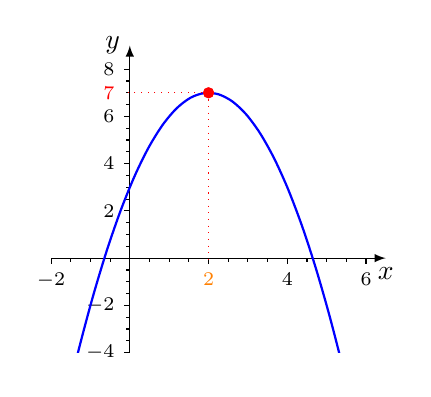
\begin{tikzpicture}[x=5mm,y=3mm,>=latex]
      \draw[thin,black,->] (-2,0) -- (6.5,0) node[below] {$x$};
      \draw[thin,black,->] (0,-4) -- (0,9) node[left] {$y$};
      % ticks:
      \foreach \x in {-2,2,4,6}
      {
        \draw[thin,black] (\x,0) -- (\x,-2pt) node[below] {$\scriptstyle\x$};
      }
      \foreach \x in {-2,-1.5,...,6.2}
      {
        \draw[thin,black] (\x,0) -- (\x,-1.5pt);
      }
      \foreach \y in {-4,-2,2,4,6,8}
      {
        \draw[thin,black] (0,\y) -- (-2pt,\y) node[left] {$\scriptstyle\y$};
      }
      \foreach \y in {-4,-3.5,...,8.2}
      {
        \draw[thin,black] (0,\y) -- (-1.5pt,\y);
      }
      \begin{scope}
        \clip (-2,-4) rectangle (6,8);
        \draw[thick,blue,domain=-2:6.5,smooth] plot (\x,{-1*(\x)^2+4*\x+3});
      \end{scope}
      \uncover<2->{%
        \draw[thin,red,dotted] (2,7) -- (-2pt,7) node[left] {$\scriptstyle7$};
        \fill[red] (2,7) circle (2pt);
      }
      \uncover<3->{%
        \draw[thin,red,dotted] (2,7) -- (2,-2pt) node[below,orange,fill=white] {$\scriptstyle2$};
        \fill[red] (2,7) circle (2pt);
      }
    \end{tikzpicture}
  \end{minipage}
  \hspace*{0.25in}
  \parbox{50mm}{%
    Here's the graph of \\
    $y = f(x)=-x^2+4x+3$
    \gap

    \uncover<2->{%
      The \emph{maximum value} or just \emph{maximum} of the function is ${\red 7}.$ 
    }
    \gap

    \uncover<3->{
      The \emph{value of $x$}\ which gives the maximum of $f(x)$ is $x={\orange 2}$
    }
    \gap

    \uncover<4->{%
      We write ${\blue f({\orange 2})} = {\red 7}$.
    }
  }
  \gap

  \uncover<5->{%
    For this example you can see this is the maximum because
    \begin{equation*}
      f(x) 
      = -x^2+4x+3
      = -(x-{\orange 2})^2+{\red 7}
    \end{equation*}
    $(x-{\orange 2})^2$ is always positive except when $x=\orange 2$\\
    {\blue so the maximum  must} be at $x=\orange 2$.
  }

}

\frame{
  \frametitle{How To Find A Maximum}

  \begin{mdframed}[style=FactStyle]
    \begin{itemize}
    \item[{\red(1)}] Find $f{\red '}(x)$

    \item[{\red(2)}] Solve $f{\red '}(x)=0.$ This is the $x$ value
      that gives the max. 

    \item[{\red(3)}] To find the maximum plug the value of $x$ found
      in {\red(2)}\ back into $f(x)$. 

    \end{itemize}
  \end{mdframed}
  \bigskip
  \pause

  \begin{enumerate}
  \item Use this method to find the maximum of $f(x) = -x^2 + 8x +5$.

    The maximum value is\ldots
    \begin{center}
      A $= 4$
      \quad 
      B $= 5$
      \quad 
      C $= -2x+8$
      \quad 
      D $= 21$
      \quad 
      E $= 15$
      \pause
      \quad
      \fbox{D}
    \end{center}
    \bigskip
    \pause

    \item Find {\red the value of $x$} which makes $f(x)=(2-x)(x+6)$ a
      maximum. 
      \smallskip

      The value of $x$ is\ldots
      \begin{center}
        A $=16$
        \quad 
        B $= 1$
        \quad 
        C $=-1$
        \quad 
        D $= 2$
        \quad 
        E $= -2$
        \pause
        \quad
        \fbox{E}
      \end{center}
  \end{enumerate}

}



\frame{
  \frametitle{How To Find A Minimum?}

  \begin{center}
    \begin{minipage}{0.4\linewidth}
      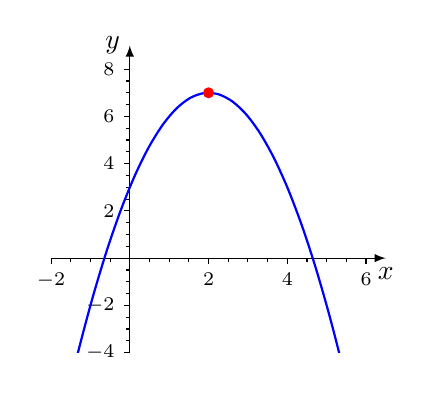
\begin{tikzpicture}[x=5mm,y=3mm,>=latex]
        \draw[thin,black,->] (-2,0) -- (6.5,0) node[below] {$x$};
        \draw[thin,black,->] (0,-4) -- (0,9) node[left] {$y$};
        % ticks:
        \foreach \x in {-2,2,4,6}
        {
          \draw[thin,black] (\x,0) -- (\x,-2pt) node[below] {$\scriptstyle\x$};
        }
        \foreach \x in {-2,-1.5,...,6.2}
        {
          \draw[thin,black] (\x,0) -- (\x,-1.5pt);
        }
        \foreach \y in {-4,-2,2,4,6,8}
        {
          \draw[thin,black] (0,\y) -- (-2pt,\y) node[left] {$\scriptstyle\y$};
        }
        \foreach \y in {-4,-3.5,...,8.2}
        {
          \draw[thin,black] (0,\y) -- (-1.5pt,\y);
        }
        \begin{scope}
          \clip (-2,-4) rectangle (6,8);
          \draw[thick,blue,domain=-2:6.5,smooth] plot (\x,{-1*(\x)^2+4*\x+3});
        \end{scope} 
        \fill[red] (2,7) circle (2pt);
     \end{tikzpicture}
    \end{minipage}
    \hspace*{0.5in}
    \begin{minipage}{0.4\linewidth}
      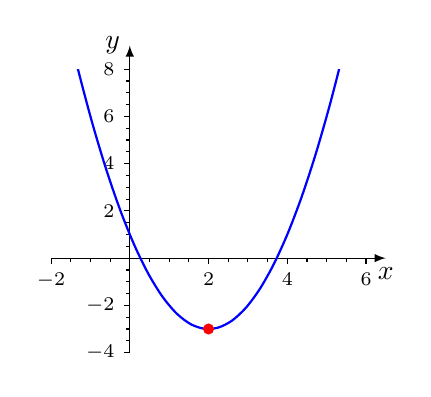
\begin{tikzpicture}[x=5mm,y=3mm,>=latex]
        \draw[thin,black,->] (-2,0) -- (6.5,0) node[below] {$x$};
        \draw[thin,black,->] (0,-4) -- (0,9) node[left] {$y$};
        % ticks:
        \foreach \x in {-2,2,4,6}
        {
          \draw[thin,black] (\x,0) -- (\x,-2pt) node[below] {$\scriptstyle\x$};
        }
        \foreach \x in {-2,-1.5,...,6.2}
        {
          \draw[thin,black] (\x,0) -- (\x,-1.5pt);
        }
        \foreach \y in {-4,-2,2,4,6,8}
        {
          \draw[thin,black] (0,\y) -- (-2pt,\y) node[left] {$\scriptstyle\y$};
        }
        \foreach \y in {-4,-3.5,...,8.2}
        {
          \draw[thin,black] (0,\y) -- (-1.5pt,\y);
        }
        \begin{scope}
          \clip (-2,-4) rectangle (6,8);
          \draw[thick,blue,domain=-2:6.5,smooth] plot (\x,{(\x)^2-4*\x+1});
        \end{scope}
        \fill[red] (2,-3) circle (2pt);
      \end{tikzpicture}
    \end{minipage}
  \end{center}
  \pause
  \bigskip

  What this technique {\blue actually does} is find both maxima and
  minima
  \smallskip

  In Math 34A a problem will have either a maximum {\red or} a
  minimum, {\red but not both}.  So the technique will find what you
  want. In Math 34B you discover how to do problems which have both a
  maximum and a minimum and find out which is which.

}

\frame{
  \frametitle{More Examples}

  \begin{enumerate}
    \setcounter{enumi}{2}
  \item What is the minimum of $f(x)=(x+2)(x+4)+3$?

    \begin{center}
      A $=0$
      \quad 
      B $ = 1$
      \quad 
      C $= 2$
      \quad 
      D $= 3$
      \quad 
      E $= 4$
      \pause
      \quad
    \end{center}
    \alert{Answer:}\ \answer{C}
    \pause
    \bigskip

    \item What is minimum of $f(x)=x^2 + 16 x^{-2}$?
      \begin{center}
        A $=2$
        \quad 
        B $= 4$
        \quad 
        C $= 6$
        \quad 
        D $= 8$
        \quad 
        E $= 16$
        \pause
      \end{center}
      \alert{Answer:}\ \answer{D}
      \pause
      \medskip

      \item Find the value of $x$ which makes $f(x)=-e^x-e^{-2x}$ a
        maximum. 
        \begin{center}
          A $=0$
          \quad 
          B $= \ln(2)$
          \quad 
          C $=-\ln(2)$
          \quad 
          D $= \ln(2)/3$
          \quad 
          E $= \ln(2)/3$
          \pause
        \end{center}
        \medskip
        \alert{Answer:}\ \answer{E}

      \end{enumerate}

}

\section{Word Problems}

\frame{ 
  \frametitle{Word Problem \#1} 

  A ball is thrown into the air. After $t$ seconds the height in
  meters above the ground of the ball is $h(t)=40t-10t^2$. How many
  meters high did the ball go?

  \begin{center}
    A $=2$
    \quad 
    B $= 40-20t$
    \quad 
    C $= 20$
    \quad 
    D $= 40$
    \pause
    \quad
    \fbox{D}
  \end{center}
  \vspace*{2in}

}


\frame{
  \frametitle{Word Problem \#2}

  If an airline sells tickets at a price of $\$200+5x$ each the
  number of tickets it sells is $1000-20x$.  What price should the
  tickets be if the airline wants to get the most money?

  \begin{center}
    A $=5$
    \quad 
    B $= 25$
    \quad 
    C $=175$
    \quad 
    D $= 200$
    \quad 
    E $= 225$
    \pause
    \quad
    \fbox{E}
  \end{center}
  \vspace*{2in}

}

\frame{ 
  \frametitle{Word Problem \#3} 

  A fenced garden with an area of $100\ \text{m}^2$  will be made in
  the shape of a rectangle. It will be surrounded on all four sides by
  a fence. What length and width should be used so the least amount of
  fence is needed? 
  \bigskip
  \pause

  \alert{Approach:}
  \begin{itemize}
  \item[{\blue(1)}] Express the total length of fence in terms of
    \emph{only}\ one variable, either $L = $ length of field, or $W =$
    width of field. This gives a formula for $P=$ (total length of
    fence) involving, say, $W$.
    \pause
    \smallskip

  \item[{\blue(2)}] Find minimum by solving $\dfrac{dP}{dW}=0$.
  \end{itemize}
  \pause
  \bigskip

  Students always find {\blue(1)}\ the hardest part.

  \alert{You}\ have been prepared for this by word problems from chapter 3!
 
  

}


\frame{
  \frametitle{Word Problem \#4 (a sequel!)}

  A fenced garden with an area of $1000\ \text{m}^2$  will be made in
  the shape of a rectangle. It will be surrounded on all four sides by
  a fence. Three sides are wood fence, and the remaining side is a
  brick wall.
  \begin{itemize}
  \item The wood fence costs \$5 per meter length.
  \item The brick wall costs \$20 per meter length.
    \pause
  \item $C=$ total cost of the fence and brick wall
  \item $L=$ length of the brick wall
  \item $W=$ width of the other side 
  \end{itemize}
  \begin{enumerate}
  \item[\colorbox{blue!50}{(a)}] Find a formula for $C$ in terms of only $L$.
    \vspace*{-0.5em}

    \begin{center}
      A $= 2W + 2L$
      \quad 
      B $= 2000L^{-1}+2L$
      \quad 
      C $= 25L +10000L^{-1}$\\[0.5em] 
      % 
      \ \quad
      D $= 20L + 10000WL^{-1}$
      \quad 
      E $= 5L + 3000$
      \pause
      \quad
      \answer{C}
    \end{center}
    % \bigskip

  \item[\colorbox{blue!50}{(b)}]
    What length of brick wall gives lowest cost?
    \vspace*{-0.5em}

    \begin{center}
      A $= 20$
      \quad 
      B $= 40$
      \quad 
      C $= 50$
      \quad 
      D $= 100$
      \quad 
      E $= 25$
      \pause
      \quad
      \answer{A}
    \end{center}
  \end{enumerate}

}

\end{document}

\frame{ 
  \frametitle{Word Problem \#5} 

  A rectangular field is surrounded by fence. It is divided into 4
  equal
  \begin{center}
    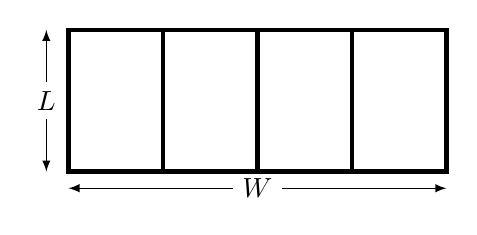
\begin{tikzpicture}[x=12mm,y=6mm,>=latex]
      \draw[thin,black,<->]  (-8pt,0) -- (-8pt,3) node[midway,fill=white] {$L$};
      \draw[thin,black,<->]  (0,-6pt) -- (4,-6pt) node[midway,fill=white] {$W$};
      \draw[ultra thick,black] (1,0) -- (1,3);
      \draw[ultra thick,black] (2,0) -- (2,3);
      \draw[ultra thick,black] (3,0) -- (3,3);
      \draw[ultra thick,black] (0,0) rectangle (4,3);
    \end{tikzpicture}
  \end{center}
  parts by 3 more dividing fences all parallel to one side of the
  field.
  % \bigskip

  \begin{enumerate}
  \item[\colorbox{blue!50}{(a)}]
    What is the total length of all the fence needed?
    \begin{center}
      A $= 2L+2W$
      \quad 
      B $= LW$
      \quad
      C $= 5LW$ \\[0.5em]
      \ 
      \quad \quad \quad 
      D $= L+W$
      \quad
      E $= 5L+2W$
      \pause
      \quad \quad \quad 
      \answer{E}
    \end{center}

  \item[\colorbox{blue!50}{(b)}]
    The field must have an area of $1000\ \text{m}^2$.
    Express $W$ in terms of $L$. 
    \begin{center}
      A\ $1000-L$
      \quad 
      B\ $1000L$
      \quad 
      C\ $1000/L$
      \quad 
      D\ $1000+L$
      \pause
      \quad
      \fbox{C}
    \end{center}
    \vspace{2in}
  \end{enumerate}

}

\frame{ 
  \frametitle{Word Problem \#5 (cont'd)}

  A rectangular field is surrounded by fence. It is divided into 4
  equal
  \begin{center}
    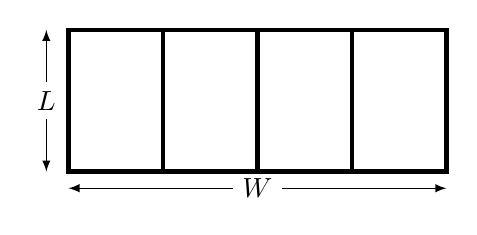
\begin{tikzpicture}[x=12mm,y=6mm,>=latex]
      \draw[thin,black,<->]  (-8pt,0) -- (-8pt,3) node[midway,fill=white] {$L$};
      \draw[thin,black,<->]  (0,-6pt) -- (4,-6pt) node[midway,fill=white] {$W$};
      \draw[ultra thick,black] (1,0) -- (1,3);
      \draw[ultra thick,black] (2,0) -- (2,3);
      \draw[ultra thick,black] (3,0) -- (3,3);
      \draw[ultra thick,black] (0,0) rectangle (4,3);
    \end{tikzpicture}
  \end{center}
  parts by 3 more dividing fences all parallel to one side of the
  field.
  \bigskip

  \begin{enumerate}
  \item[\colorbox{blue!50}{(c)}]
    Express the total length of all the fence needed in terms of $L$.
    \begin{center}
      A $= 5L+1000$
      \quad 
      B $=  5L + 2000/L$
      \quad 
      C $= 5L+2/L$
      \quad
      \pause
      \answer{B}
    \end{center}

  \item[\colorbox{blue!50}{(d)}]
    What should $L$  be so that the total length of fence used is a minimum?
    \begin{center}
      A $=10$
      \quad 
      B $=20$
      \quad 
      C $= 40$
      \quad 
      D $= 50$
      \pause
      \quad\answer{B}
    \end{center}
  \end{enumerate}
    \vspace*{2in}
}






\end{document}
